%%%%%%%%%%%%%%%%%%%%%%%%%%%%%%%%%%%%%%%%%%%%%%%%%%%%%%%%%%%%%%%%%%%%%%%%%%%%%%%%
%2345678901234567890123456789012345678901234567890123456789012345678901234567890
%        1         2         3         4         5         6         7         8

\documentclass[letterpaper, 10 pt, conference]{ieeeconf}  % Comment this line out
                                                          % if you need a4paper
%\documentclass[a4paper, 10pt, conference]{ieeeconf}      % Use this line for a4
                                                          % paper

\IEEEoverridecommandlockouts                              % This command is only
                                                          % needed if you want to
                                                          % use the \thanks command
\overrideIEEEmargins
% See the \addtolength command later in the file to balance the column lengths
% on the last page of the document



% The following packages can be found on http:\\www.ctan.org
\usepackage{graphicx} % for pdf, bitmapped graphics files
%\usepackage{epsfig} % for postscript graphics files
%\usepackage{mathptmx} % assumes new font selection scheme installed
%\usepackage{times} % assumes new font selection scheme installed
%\usepackage{amsmath} % assumes amsmath package installed
%\usepackage{amssymb}  % assumes amsmath package installed


\title{\LARGE \bf
CS 4758 Robot Learning: Beer Pong Butler
}

%\author{ \parbox{3 in}{\centering Huibert Kwakernaak*
%         \thanks{*Use the $\backslash$thanks command to put information here}\\
%         Faculty of Electrical Engineering, Mathematics and Computer Science\\
%         University of Twente\\
%         7500 AE Enschede, The Netherlands\\
%         {\tt\small h.kwakernaak@autsubmit.com}}
%         \hspace*{ 0.5 in}
%         \parbox{3 in}{ \centering Pradeep Misra**
%         \thanks{**The footnote marks may be inserted manually}\\
%        Department of Electrical Engineering \\
%         Wright State University\\
%         Dayton, OH 45435, USA\\
%         {\tt\small pmisra@cs.wright.edu}}
%}

\author{Kimberly Sheriff, kgs45, and Brian Toth, bdt25}


\begin{document}



\maketitle
\thispagestyle{empty}
\pagestyle{empty}


%%%%%%%%%%%%%%%%%%%%%%%%%%%%%%%%%%%%%%%%%%%%%%%%%%%%%%%%%%%%%%%%%%%%%%%%%%%%%%%%
\begin{abstract}

This paper describes the application of the PR2 robot as a ''Beer Pong Butler", which will identify a ping pong ball in a cup, pick up that cup, and move it to another location. We utilize Hough’s circle detection using OpenCV and an SVM to detect a ball in a cup. We then use motion planning to perform the task given the location of the cup containing a ball.

\end{abstract}


%%%%%%%%%%%%%%%%%%%%%%%%%%%%%%%%%%%%%%%%%%%%%%%%%%%%%%%%%%%%%%%%%%%%%%%%%%%%%%%%
\section{Introduction}

Beer pong, also known as Beirut, is a drinking game typically played at college parties, which involves two teams of two players each throwing ping pong balls across a table with the goal of sinking a ball into a cup of beer at the other end. Figure ~\ref{fig:pongtable}, shows the typical set up for a beer pong game. For our application, we will assume a game played with six cups on each side, which will be empty for our purposes. 

When a ball is successully thrown into a cup, that cup must be removed from the game. The beer pong butler will identify the cup that contains a ball and move that cup away from play.

\begin{figure}[thpb]
      \centering
	  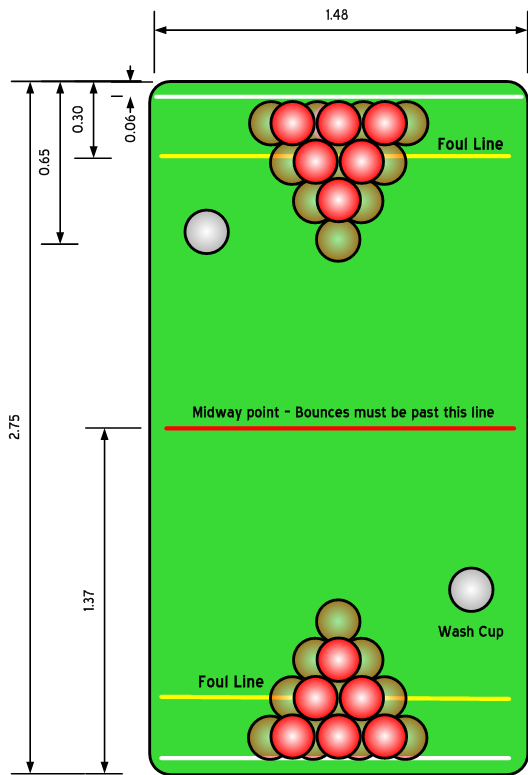
\includegraphics[scale =0.25]{pongtable}
      \caption{Typical beer pong setup.}
      \label{fig:pongtable}
\end{figure}

\subsection{Related Work}

Willow Garage has implemented a PR2 which responds to a "Beer Me" app that allows users to request a beer be brought to them from the fridge. The PR2 navigates to the fridge, uses handle recognition to open the door, and object recognition to determine which beers are in a rack in the fridge. The fridge is modeled using live perception and data from several sources according to a representative from Willow Garage. The PR2  uses motion planning, presumably some type of inverse kinematic solver, to determine the path of the arm to the beer to be picked up.The PR2 is also capable of opening the beer bottle. This algorithm provides the makings of a full service party bot, and our application attempts to provide additional functionality.  

Solem’s Vision Blog explains how to use Hough’s transforms and OpenCV to detect lines and circles on an image of a guage. HoughCircles is a documented function in python which takes as input: the image, the detection method to use, the inverse ratio of the accumulation resolution to the image resolution, minimum distance between the centers of the detected circles, two threshold values, and the minimum and maximum radii. These parameters must be tweaked for different applications.

SVMs are becoming widely used for image classification. David et al. use SVM to genetic syndrome diagnosis which requires image classigication. The results shown in Table 6 of their report shows a comparison between the error rates of the SVM to other machine learning algorithms including 7-nearest neighbor, neural network, and naive bayes. The results show that SVM has the lowest error rate of the compared algorithms. Anthony et al. use SVM for land cover mapping. Their results show high accuracy using both one-versus-one and one-versus-all approaches, and they conclude that the choice between the two methods for image classification is simply personal preference.

\section{Approach}

From a high level, our approach is to detect the remaining cups, determine which cup has a ball in it, find the X,Y, and Z coordinates of that cup in the base\_link\_frame, and remove that cup from the formation.  This involves learning what a cup looks like and planning motion to a specified point.

\subsection{Perception}

The most complicated and novel part of our project is detecting which cup contains a ball.  Although this sounds simple at first, it rapidly becomes complicated when the possibilities of changing environments, lighting, cups, and viewing angles are considered.

\subsubsection{Tabletop Detection}

Most of our effort was expended attempting to segment the tabletop from the objects on the table.  Although we were successful in doing so, the resulting pointcloud was not dense enough to actually determine which cup contained the ball.  To solve this, we are currently in the process of overlaying the pointcloud data on the rbg image, with mixed results.

The purpose of detecting the tabletop and removing it from consideration is to isolate the pixels which form the triangle of cups.  Although the image segmentation is not fine-grained enough to detect individual cups, the task of picking out cups from the RBG image is greatly simplified when the image can be cropped to a "blob" which closely follows the cups.

\begin{figure}[thpb]
      \centering
	  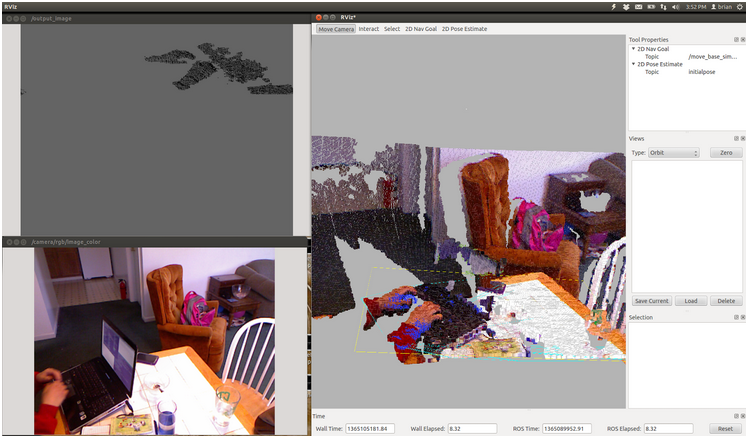
\includegraphics[width = 0.5\textwidth]{detect}
      \caption{Table top detection with pointcloud and rgb image data.}
      \label{fig:detect}
\end{figure}

Shown here (clockwise from the right) are the registered pointcloud, the rbg image, and one result of tabletop segmentation projected onto a two dimensional image.  Tabletop segmentation returns significant clusters of points which appear above the tabletop surface.  In this case, one such cluster is the hands and keyboard of the person working at the computer.  The cluster is not yet properly aligned with the RBG image because we have not yet determined which method of coordinate transform is necessary to transform from the Kinect's 3D coordinate frame to its 2D coordinate frame.  Methods attempted include using ROS's tf, projecting the 3D coordinates on to the plane of the observer and rotating that plane, converting the pointcloud to an image directly using ROS's CloudToImage, and simply removing the Z coordinate of each point (most successful, pictured).


\subsubsection{Cup Detection}

We considered a number of alternatives for using machine learning to bolster perception.  Although openCV’s Hough Circles do a good job of delimiting cups when properly tuned, as shown in Figure ~\ref{fig:positive}, they can perform erratically when the parameters are a bit off.  Slight changes in environment, lighting, height, or angle can result in incorrect or incomplete labeling of cups as seen in Figure ~\ref{fig:negative}.

\begin{figure}[thpb]
      \centering
	  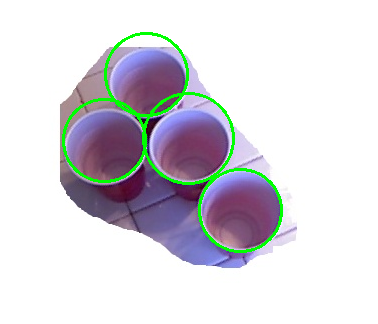
\includegraphics[scale =0.5]{4_cups}
      \caption{Positive example with all cups labeled correctly.}
      \label{fig:positive}
\end{figure}

\begin{figure}[thpb]
      \centering
	  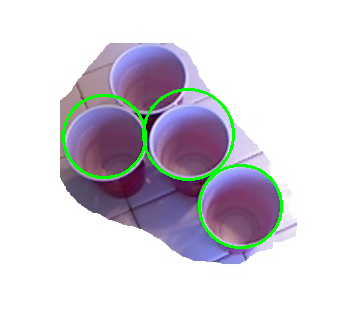
\includegraphics[scale =0.5]{4_cups_bad}
      \caption{Negative example with cup 6 not captured.}
      \label{fig:negative}
\end{figure}

Our first idea was to implement a combined HMM and SVM to determine whether we had properly identified the cups.  The problem naturally lends itself to an HMM, because there are a small number of discrete states (configurations of the cups), and the game naturally transitions from one state to another.  Even better, the transition probabilities are certainly not uniform and can be determined experimentally simply by throwing balls into cups.  Although we were very excited about this approach, it was abandoned due to time constraints.  Because each unique configuration would require a custom SVM to be trained, there would have to be 6+6+15+15+20+1+1= 64 different SVMs.  Gathering sufficient data to train and validate this many SVMs would not be practical.

Instead, we are pursuing three different, simpler classifiers which will be compared against our dataset to determine which performs the best.  The ultimate evaluation is the ability to detect if the ball is present and, if it is, where it is located.

The simplest classifier simply looks to determine, for each drawn circle, if that circle represents a valid cup.  Therefore this classifier considers only one cup at a time.  Features include the radius of the circle and the average color of pixels in the circle.  The number of detected cups (and the probability of each circle being a cup) is fed into a simple HMM.  Unlike the HMM mentioned previously, this HMM contains only six states, one for each possible total number of cups.  At each time update, the HMM can either transition to the next state (remove a cup) or keep the same number of cups.  This is used as a sanity check for the circle detector; if the identified number of cups is not equal to the expected number of cups or one fewer than the detector is re-run with different parameters.

The second classifier takes a slightly different approach by considering all of the detected cups at once. Adding the number of cups detected and the number of cups expected as features along with color data for each cup, allows the entire set of circles to be accepted or rejected at once.  This increases the amount of information which can be learned, but has the disadvantage of requiring more guesswork during training (we have to make assumptions about the expected number of cups).

The final classifier goes even further in attempting to consider the entire formation of cups by adding additional features to represent the implicit information in the HMM model.  The first six features represent the “best fit” that the Hough Circle detector can perform given the circles it finds.  Currently the assignment of numbers to cups is done by comparing to the initial 6 cup pyramid.  This makes the assumption that the robot does not significantly move during the course of the game; we are also pursuing an ‘absolute’ model based on coordinates.
    
The information from the “previous state” is incorporated in features 26-31.  Assuming the robot successfully removed a cup in the previous iteration and all of the circles were detected properly, this will match features 1-6 exactly.

The other features are currently experimental attempts to characterize a cup.  This SVM is really doing double-duty; it requires both the detection of the correct number of cups in the correct relative positions and that the circles detected are actually cups.  At present we average the rbg values of the pixels within the cup-circles.\\\\
Features: 
$1 \rightarrow 6$: did the cup detector find cup x. \\
$7 \rightarrow 25$: average rgb values for cups\\
$26 \rightarrow 31$: was the cup there (i.e. should the cup detector have found cup x)\\

Sample feature vector:\\

$1  <1:0 2:1 3:0 4:0 5:0 6:0 7:146.605410924 8:121.33146163 9:135.208269525 .... 26:0 27:1 28:0 29:0 30:0 31:0>$ \\


All of the above use the same method to actually find the ball.  Each identified cup is passed to another SVM which is specifically trained to identify the cup which has the ball.  The features for this SVM are the average color for the cup and the number of orange-like pixels.  This process is separate from the task of actually finding cups, because, until the entire formation is identified, there is little point in searching for the ball.

\begin{figure}[thpb]
      \centering
	  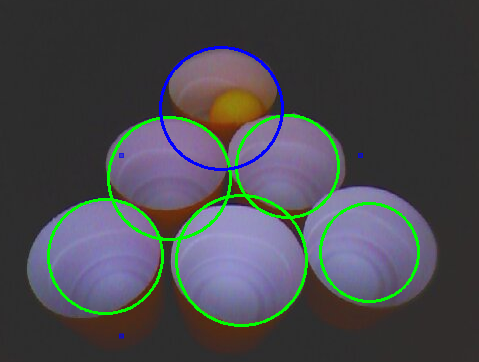
\includegraphics[width = 0.5\textwidth]{ball_detected_6}
      \caption{Detecting the presence of a ball using previously identified cups}
      \label{fig:ball_detected}
\end{figure}

\subsection{Motion Planning}

We began by working with pick and place, but this algorithm does not work for our application because we are not picking up a stand alone object. We proceeded to investigate other motion planning techniques including an inverse kinematic solver. Given the x,y,z location of the center of the desired cup, our goal was to move the gripper three inches above that location. The three inches would allow room to rotate the gripper such that it is oriented downward into the cup. The gripper would then be move five inches downward so that the gripper is inside the cup near the center. The gripper would then spread, securing the cup. This method of gripping the cup was determined to be the best because it could be used on any cup whether it is on an edge or surrounded by other cups. We would then raise the arm to remove that cup from the game.  This approach proved problematic due to sensitivity of the inverse kinematic solver. 

The first step taken was to successful run the move\_arm\_pose\_goal tutorial. This tutorial takes a set of position and orientation coordinates and solves inverse kinematics to determine the path to move the end effector to that position. Next, we looked at the position of the coke can in the pr2\_gazebo world launched from pr2\_table\_object.launch. The coke can is at position x = 0.7, y = 0, z = 0.55. We then plugged these coordinates into our inverse kinematic solver but it failed. We guessed that this might have failed because if the end effector moved to those coordinates it would be colliding with the coke can, so we tried the same coordinates in the world launch by pr2\_empty\_world.launch. The inverse kinematics again failed, and we began changing the coordinates small amounts in each direction in attempt to get the inverse kinematics to solve. The idea was that the location of the coke can was difficult for the PR2 to navigate to (not impossible) and the sensitivity of the PR2 found joints violating limits. We were unable to successful use inverse kinematics to move the arm to the desired position.

We use a model of the red plastic cups which was found on the Google 3D warehouse. We are in the process of creating a launch file which will spawn a table and six of the downloaded cups in the correct orientation.


\section{Experiments}

Because our project revolves around detecting which cup has the ball and moving to those XY coordinates

\subsection{Setup}

\subsection{Data}

Our data set is comprised of 51 images taken with the Kinect. We label the cups one to six from left to right starting at the bottom left corner. The images were taken of various configurations of the cups, removing different sets of cups or no cups for each image. The angle and position of the Kinect relative to the cup arrangement was also varied as was the lighting.  A few different red plastic cups were used for the images. 

\subsection{Evaluation Metric}

The ultimate evaluation metric is the ability to detect the ball.  Although many of our methods revolve around detecting cups, this is only an intermediary step.  Thus each image is labeled to indicate the coordinates of the ball (negative coordinates indicate that there is no ball present).  An algorithm succeeds if it selects a point near the ball.

\subsection{Results}

Unfortunately we do not yet have any results for our experiments.  Although we have collected data and are currently implementing multiple learning algorithms, we have not yet run these on the full data set.


\section{Future Work}

\subsection{Motion Planning}
We are considering using the ee\_cart\_imped package as part of our motion planning. The advantage and disadvantage to using ee\_cart\_imped is that it does not take into account possible collisions. This is an advantage because it will be less senstitive than working with inverse kinematics and might be more successful. It is a disadvantage because it may very easily knock over other cups or hit something on its trajectory. We also plan to continue work with the inverse kinematic solver. We plan to consult with a TA to determine the best approach going forward.

Another current issue is that our perception work is done using the coordinate system of the Kinect whereas our motion planning is down in the base\_link coordinate system. We will need to determine a coordinate transform before combining our motion planning and perception.

\subsection{Perception}
Our perception algorithms need to be tested by running cross validation and evaluating our learning algorithms. We have created a data set as described, and that data set should be split in order to be used to train, test, and evaluate.





\begin{thebibliography}{99}

\bibitem{c1} "Beer Me, Robot." Willow Garage. N.p., n.d. Web. 05 Apr. 2013.
\bibitem{c2} "Feature Detection¶." Feature Detection — OpenCV 2.4.4.0 Documentation. N.p., n.d. Web. 05 Apr. 2013.
\bibitem{c3} http://www.janeriksolem.net/2012/08/reading-gauges-detecting-lines-and.html
\bibitem{c4} Anthony, Gregg, and Tshilidzi. Image Classification Using SVMs: One-against-One Vs One-against-All. Tech. N.p.: n.p., n.d. Print.
\bibitem{c5} David, and Lerner. Support Vector Machine-based Image Classification for Genetic Syndrome Diagnosis. Tech. N.p.: n.p., n.d. Print.







\end{thebibliography}




\end{document}
